\part{Preliminaries}\label{part:Introduction}

% 介绍SIFT的提出背景与Harris的区别,先验知识
对图像底层的局部特征进行检测和描述是解决很多计算机视觉问题的基础,例如物体识别、图像匹配和图像复原。在对这些局部特征进行匹配后,算法就能够对不同视角图像当中的特殊区域进行识别和比较。

在图像底层局部特征提取的诸多算法当中,\sift 是迄今使用最为广泛的一种特征,它具有以下优点:
\begin{itemize}
	\item \rinvariance 和\sinvariance :对图像的旋转和尺度变化具有不变性;
	\item 对三维视角变化、光照变化以及噪声具有很强的适应性;
	\item 在存在遮挡或场景杂乱的情况下,底层的局部特征具有不变性;
	\item 辨别力强:特征之间相互区分的能力强,有利于匹配;
	\item 扩展性强:能够与其他形式的特征向量联合
	\item 易获取:一般$500\times 500$的图像能提取出约2000个特征点
\end{itemize}

下面对\sift 背后的原理进行简单论述。

\section{LoG的空间选择特性}

回忆当我们在进行边缘检测时,会使用\gspd 对图像做卷积,得到的图像与在原图像基础上先后进行\emph{高斯平滑}与\emph{求导}两个操作等价,最终响应值最高处即被确定为边缘所在位置。

其实,高斯二阶导也可用于边缘检测。高斯二阶导也被叫做\lpl ,与之卷积所获得的图像与在原图像基础上先后进行\emph{高斯平滑}与\emph{连续求二阶导}两个操作等价,最终响应值过零点处即被确定为边缘所在位置。

\begin{marginfigure}
	\centering
	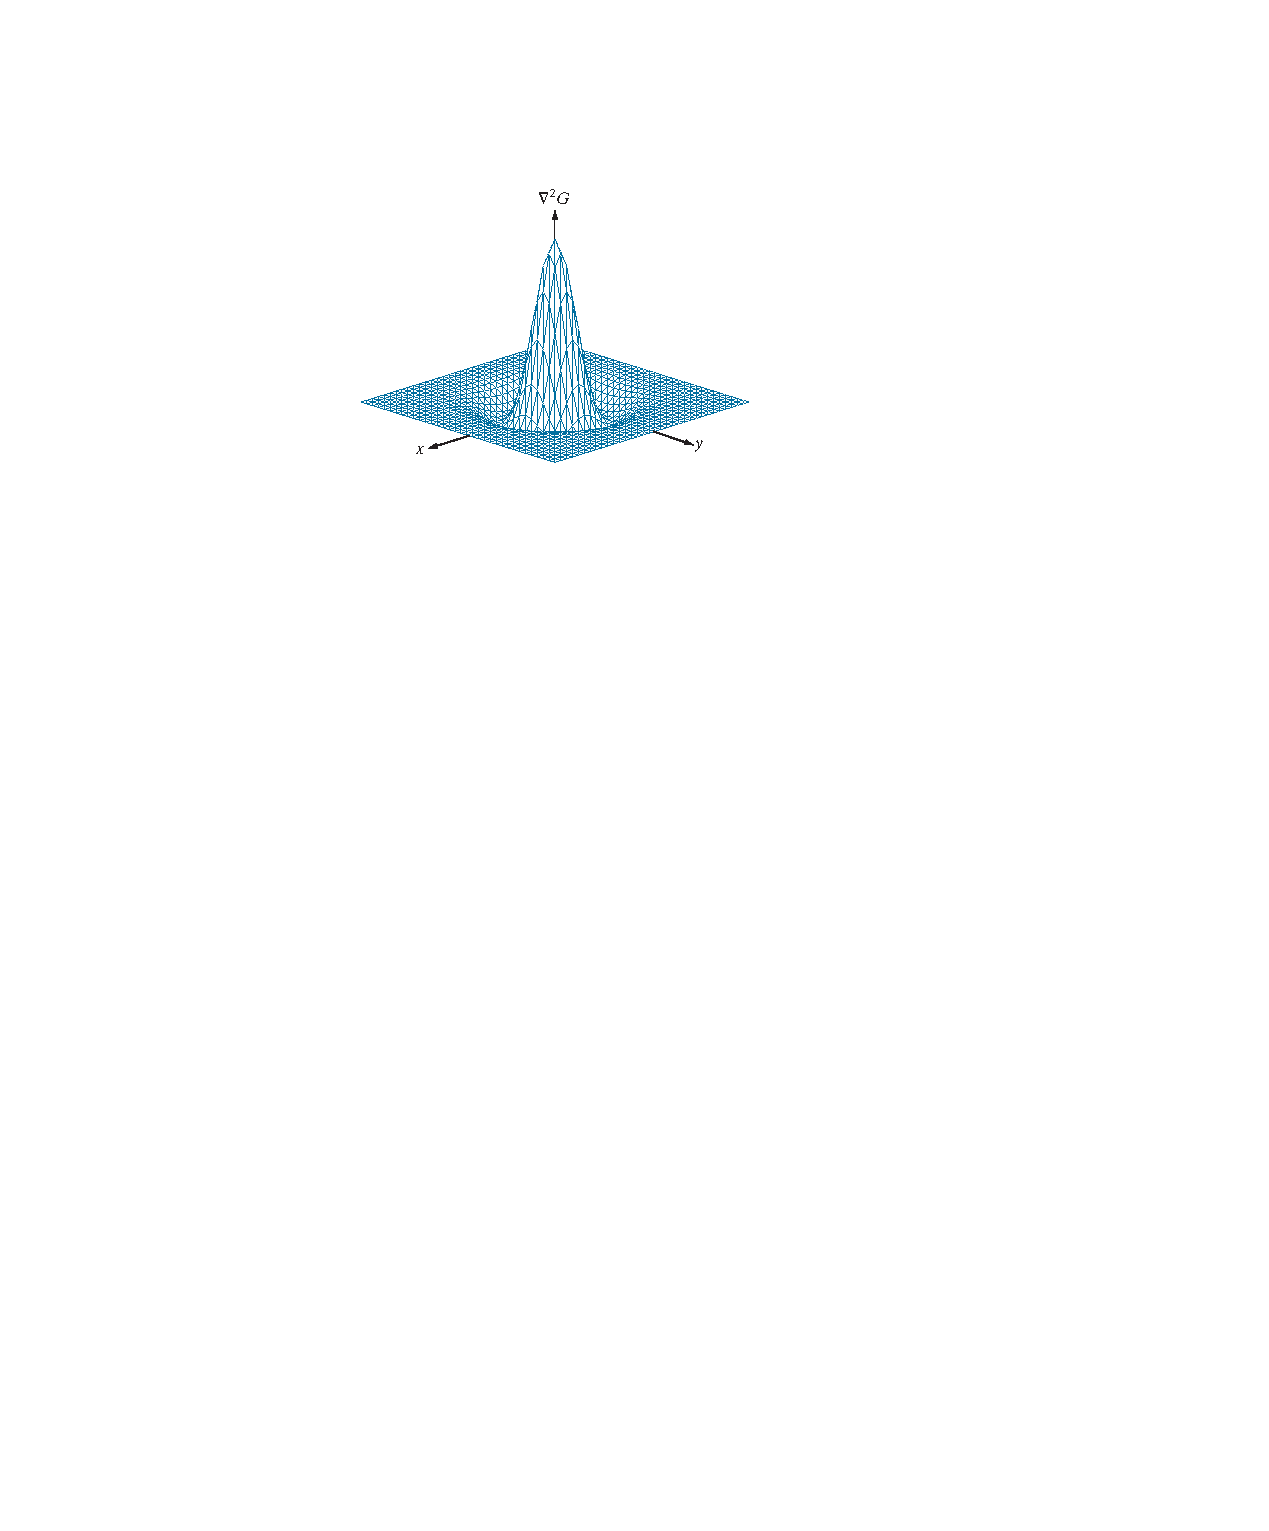
\includegraphics[width=\textwidth]{fig/LoG.pdf}
	\caption{3-D plot of the negative of the LoG.}
\end{marginfigure}

\begin{figure}[H]
	\centering
	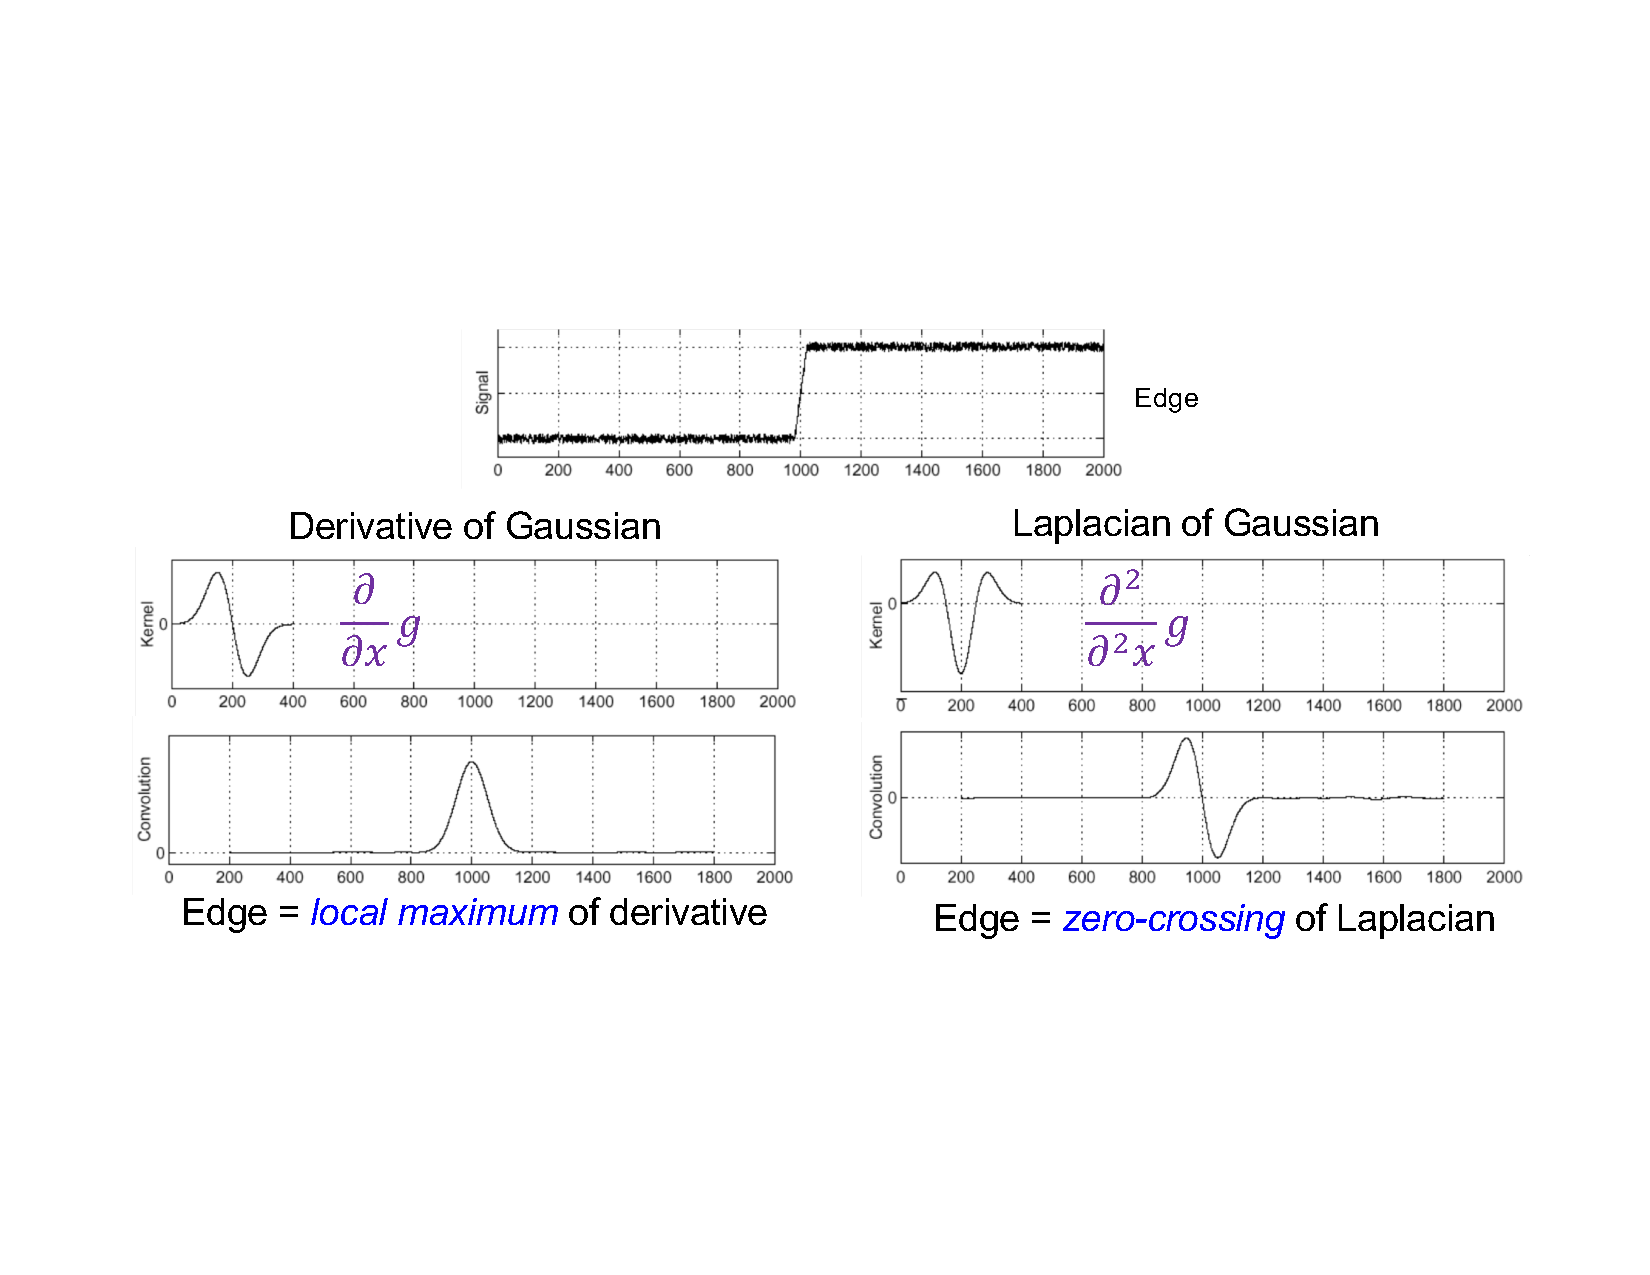
\includegraphics[width=.9\textwidth]{fig/Edge detection with LoG.pdf}
	\caption{\gspd 和\lpl 分别进行边缘检测\cite{marr1980theory}。}
\end{figure}

不仅如此,\lpl 相比于\gspd 还拥有一个更好的特性,即具有\emph{空间选择特性(Spatial Selection)}:% 插图
当\lpl 的尺度$\sigma$与信号的宽度匹配时,两者卷积会在原信号的中心位置有最大响应。

\begin{figure}[H]
	\centering
	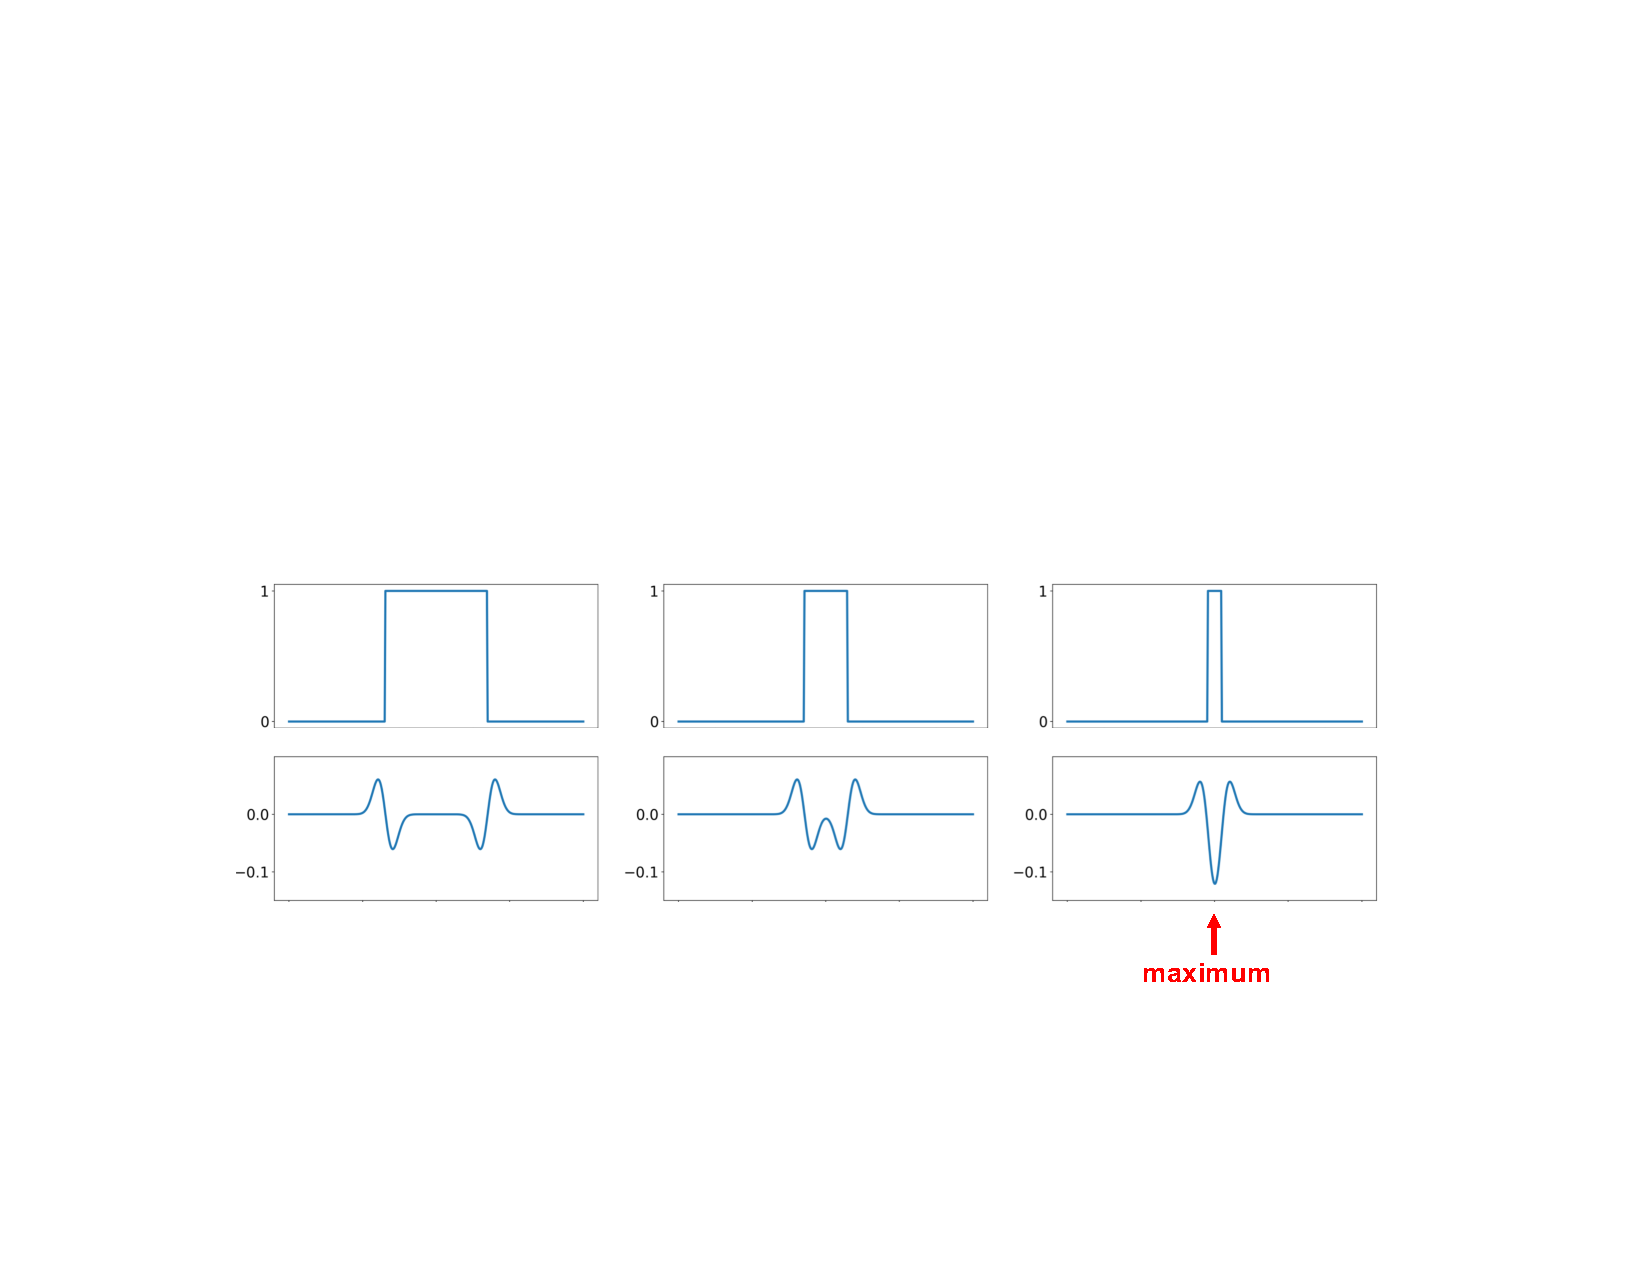
\includegraphics[width=.9\textwidth]{fig/spatial selection.pdf}
	\caption{\lpl 具有空间选择特性。}
\end{figure}

因此容易想到由\lpl 的空间选择特性,用一组尺度不一的\lpl 分别与某一尺度未知信号做卷积,通过判断响应值的大小最终确定该信号的尺度。而响应值最大时\lpl 与信号在尺度上到底存在什么数量关系呢?

\begin{marginfigure}
	\centering
	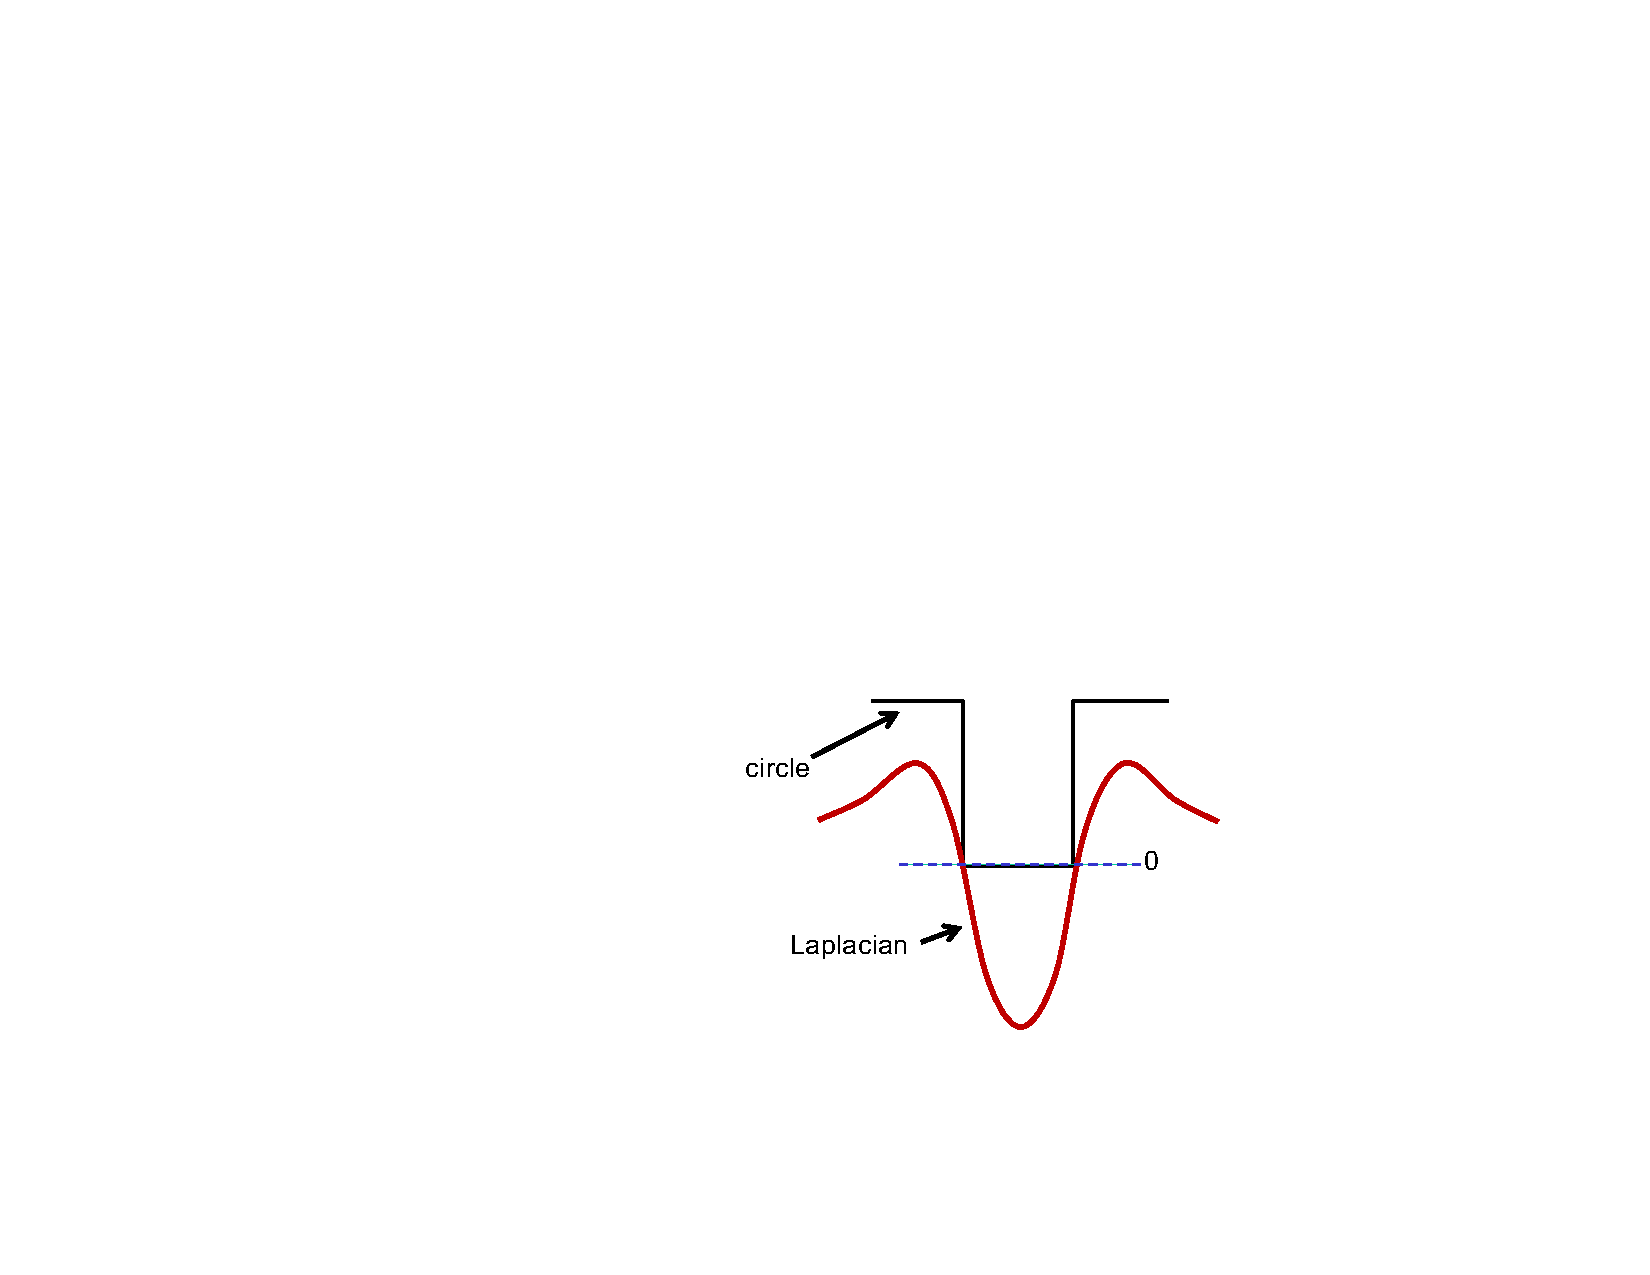
\includegraphics[width=\textwidth]{fig/LoG zero crossings-2.pdf}
	\caption{\lpl 的过零点刚好与信号卡住的情形。}
\end{marginfigure}

\begin{intu}
	当\lpl 的过零点刚好与信号卡住的时候,会在信号的中心点产生最大响应。于是,令
	\begin{equation*}
		\nabla^2_{\text{norm}}g = 0
	\end{equation*}
	得到$x^2+y^2=2\sigma^2$,即要想产生最大响应,信号的半径$r$应等于\lpl 过零点围成的半径$\sqrt{2}\sigma$。换句话说,与半径为$r$的信号产生最大响应的\lpl 参数$\sigma$应当满足:$\sigma=r / \sqrt{2}$。
	% TODO
	\begin{figure}[H]
		\centering
		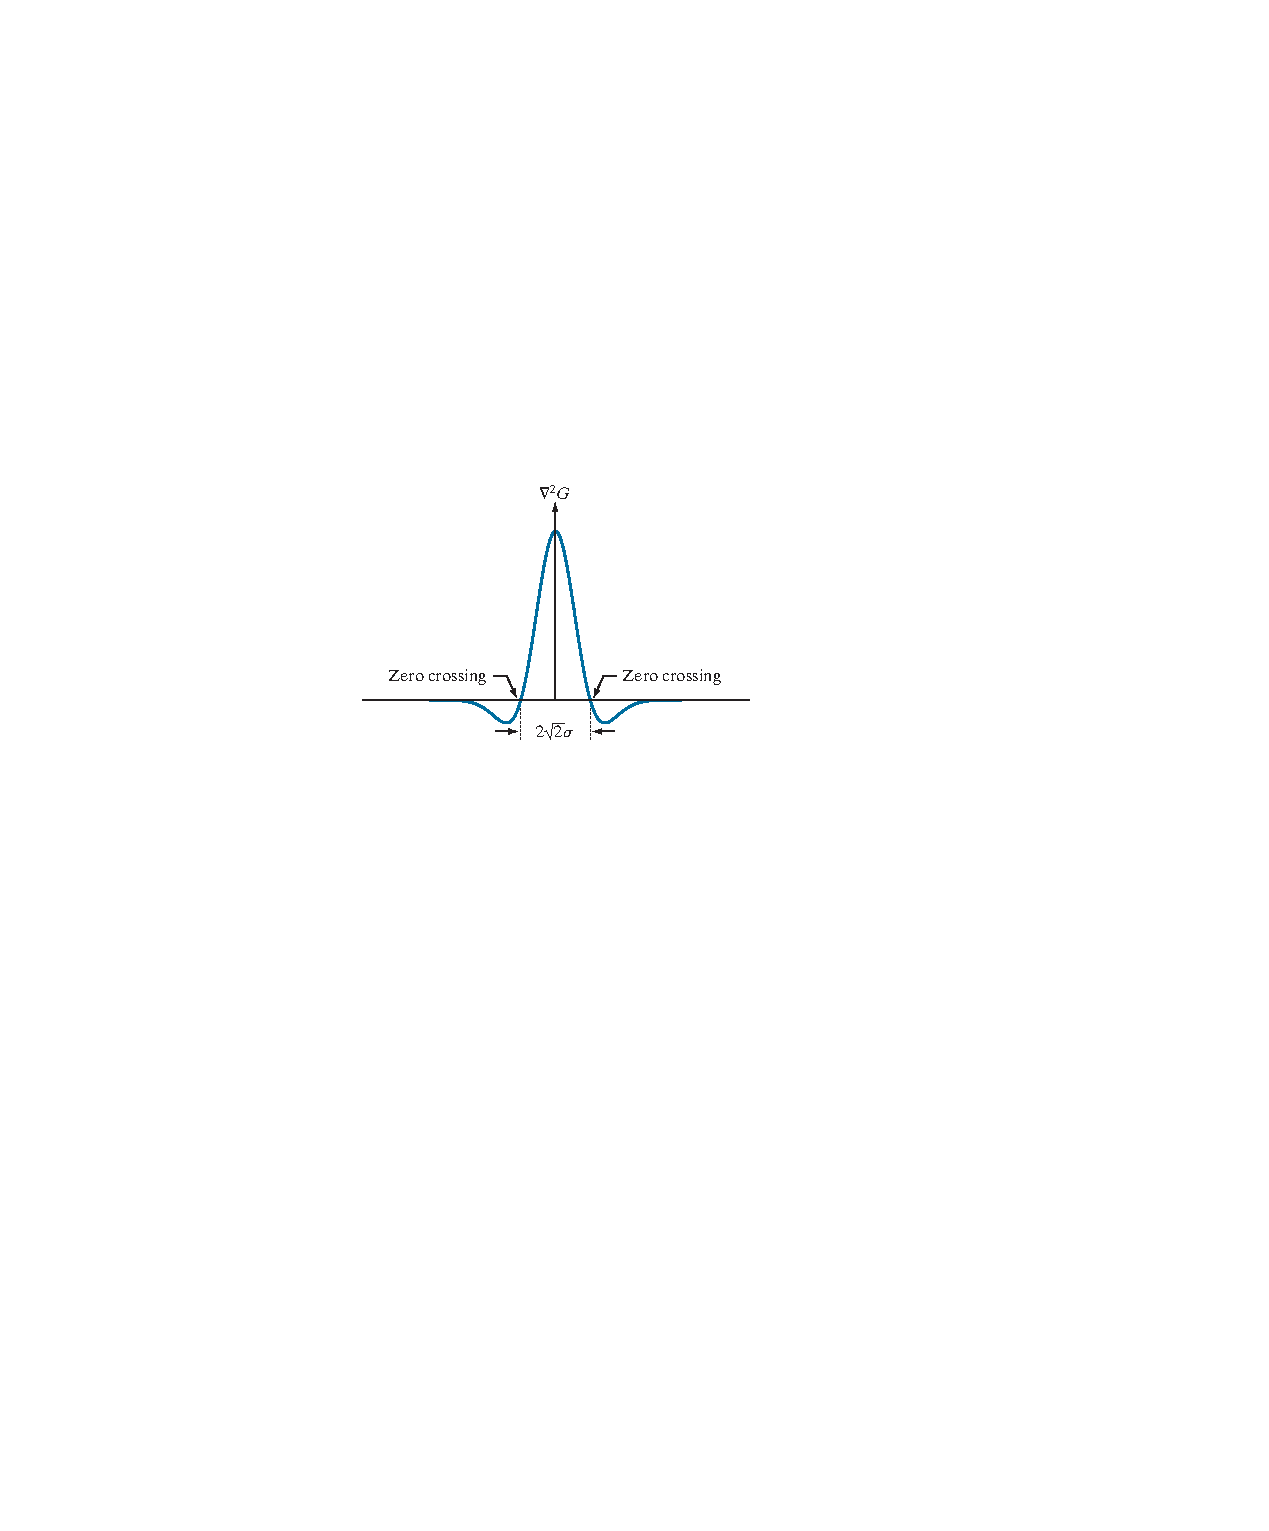
\includegraphics[height=6cm]{fig/LoG zero crossings.pdf}
		\caption{\lpl 过零点}
	\end{figure}
\end{intu}

直觉上看,信号的尺度和与之产生最大响应值的\lpl 的$\sigma$存在上述关系。但事实上,卷积的响应值会随着尺度$\sigma$的增大不断衰减,因此在此之前还必须对响应值进行\emph{尺度补偿(scale normalize)}:
\begin{equation}
	\nabla^2_{\text{normalized}}g=\eqnmarkbox[emph2]{compensate}{\sigma^2}\left(\frac{\partial^2 g}{\partial x^2} + \frac{\partial^2 g}{\partial y^2}\right)
\end{equation}

\section{图像尺度空间}

对于图像信号,如果希望找到图像上以某一点为中心所在局部特征的尺度$r$,就可以使用一组尺度($\sigma$)不同的归一化\lpl 分别对图像做卷积。\figref{fig:Scale-space blob detector}表示了一组用多尺度\lpl 相卷积得到的图像尺度空间,%
在纵向找到该位置处响应值最大时的\lpl,然后根据其参数$\sigma$即可计算局部特征的尺度$r = \sqrt{2}\sigma$。%
\begin{marginfigure}
	\centering
	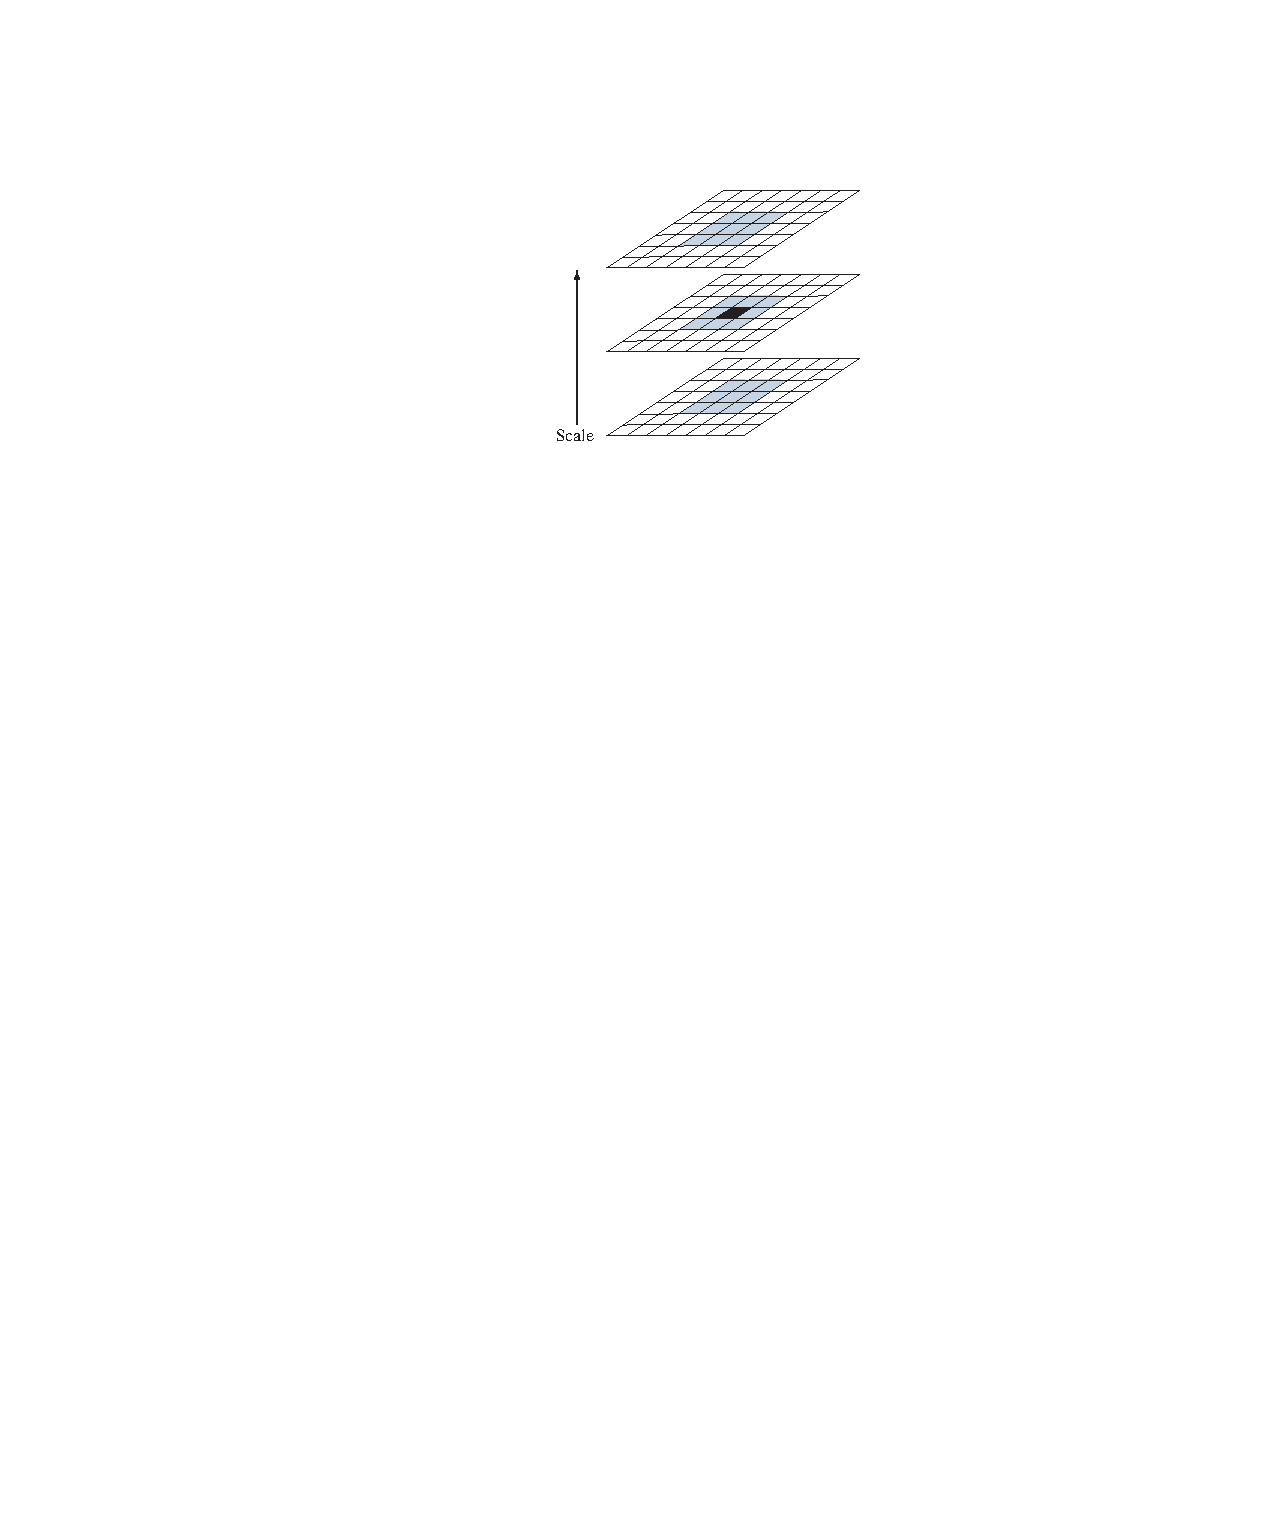
\includegraphics[width=\textwidth]{fig/Scale-space blob detector.pdf}
	\caption{图像尺度空间特征检测}
	\label{fig:Scale-space blob detector}
\end{marginfigure}


要对图像提取局部特征时,就对每一个像素坐标进行上面的操作。但是实际中并不会将\lpl 组的尺度划分得过细以逼近响应极值,这样将造成过大的计算消耗,同时意味着每一个像素坐标只能对应一个局部特征。因此,通常每三个\lpl 尺度进行比较,如果中间的响应值大于上下,则认为中间这个位置为响应极值,从而可确定出其所对应局部特征的尺寸。

然后横向在响应极值所在的尺度平面上看,周围像素其对应的响应也可能是极值,这也就导致了图像中局部特征可能会大量重叠。因此还需要进行\emph{非极大值抑制},其思路就是在确定响应极值时,不仅纵向跟自己位置进行比较,还需要跟图像尺度空间当中周围的26个像素相比,如果该响应值仍然最大,则保留这一处这一尺度的局部特征,否则遗弃该位置。

至此介绍了在图像尺度空间进行\emph{尺度搜索}和\emph{非极大值抑制}两个关键环节。但是上述过程仍然需要进行大量计算,为此\cite{mikolajczyk2001indexing}提出了Harris-Laplacian方法,先找出图像当中所有的Harris角点,然后只在这些点周围建立尺度空间,进行\lpl 的尺度分析。Harris对光照、平移、旋转具有不变性,再加上\lpl 的空间选择特性带来具有尺度不变性的局部特征。再到后来\cite{lowe2004distinctive}提出了更加高效的\sift 特征提取方法。
